\section{Airplane Landing Problem}
 Let $x_1, x_2,...,x_n $ be the exact landing time of each airplane respectively, the problem can be written as 
 \[	\begin{split} 
	 \max  \quad &\min(x_2 - x_1, x_3 - x_2, ..., x_n - x_{n-1}) \\
	\text{s.t.} \quad & s_i \leq x_i \leq t_i, i = 1,2,\cdots, n\\
	\end{split}  
 \]
 LP form
 \[
	\begin{split} 
	\max  \quad &d \\
	\text{s.t.} \quad & s_i \leq x_i \leq t_i, i = 1,2,\cdots, n\\
	& x_k - x_{k-1} \geq d, k = 2,3,\cdots, n \\
	&d \geq 0
	\end{split}  
 \]
 Now we show that how to obtain the dual form of this question,
 first we minimize $-d$,
 \[
	 \begin{split} 
	 \min  \quad &z = -d \\
	 \text{s.t.} \quad & s_i \leq x_i \leq t_i, i = 1,2,\cdots, n\\
	 & -x_{k+1} + x_{k} \leq -d = z, k = 1,2,\cdots, n-1 \\
	 &z \leq 0
	 \end{split}  
 \]
 using Lagrange multiplier, 
 \[
	 L(z, x, \lambda, \alpha, \varphi,\phi) = 
	 z + \sum_{i=1}^{n} \lambda_i (x_i - t_i) + 
	 \sum_{i=1}^{n} \alpha_i (-x_i + s_i) + 
	 \sum_{i=1}^{n-1} \varphi_i (-x_{i+1} + x_i - z) + \phi z
 \]
 \[
	\begin{split}  
	 \frac{\partial L}{\partial z} &= 1 - \sum_{i=1}^{n-1} \varphi_i + \phi = 0 \\
	 \frac{\partial L}{\partial x_1} &= \lambda_1 - \alpha_1 + \varphi_1 = 0  \\
	 \frac{\partial L}{\partial x_n} &= \lambda_n - \alpha_n - \varphi_{n-1} = 0 \\
	 \frac{\partial L}{\partial x_i} &= \lambda_i - \alpha_i + \varphi_i - \varphi_{i-1} = 0, i = 2,3,\cdots, n-1 
	 \end{split} 
 \]
 thus
 \[ \begin{split} 
	 g(\lambda,\alpha,\varphi, \phi) &= \inf_{z,x} L(z,x,\lambda, \alpha, \varphi, \phi)  \\ 
	 &= z(1 - \sum_{i=1}^{n}\varphi_i+ \phi)  + x_1(\lambda_1 - \alpha_1 + \varphi_1) + x_n(\lambda_n - \alpha_n - \varphi_{n-1}) + \\
	 &\quad \sum_{i=2}^{n-1} x_i(\lambda_i - \alpha_i + \varphi_i - \varphi_{i-1})
	 - \sum_{i=1}^{n}\lambda_i t_i + \sum_{i=1}^{n} \alpha_i s_i \\
	 &= - \sum_{i=1}^{n}\lambda_i t_i + \sum_{i=1}^{n} \alpha_i s_i
	 \end{split}
 \]
 Minimizing $-d$ is equivalent to 
 \[
	 \begin{split} 
	 \max \quad &- \sum_{i=1}^{n}\lambda_i t_i + \sum_{i=1}^{n} \alpha_i s_i \\
	 \text{s.t.} \quad&  \lambda_i \geq 0, \alpha \geq 0, i = 1,2,\cdots, n \\
	 &\varphi_i \geq 0, i = 1,2,\cdots, n-1\\
	  &\lambda_1 - \alpha_1 + \varphi_1 = 0 \\
	  &\lambda_n - \alpha_n -\varphi_{n-1} = 0\\
	  & \lambda_i - \alpha_i + \varphi_i - \varphi_{i-1} = 0, i = 2,3,\cdots,n-1\\
	  &1 - \sum_{i=1}^{n-1} \varphi_i \leq 0
	 \end{split} 
 \]
 Hence the original problem that Maximizing $d$ is equivalent to
 \[
 \begin{split} 
 \min \quad & \sum_{i=1}^{n}\lambda_i t_i - \sum_{i=1}^{n} \alpha_i s_i \\
 \text{s.t.} \quad&  \lambda_i \geq 0, \alpha_i \geq 0, i = 1,2,\cdots, n \\
 &\varphi_i \geq 0, i = 1,2,\cdots, n-1\\
 &\lambda_1 - \alpha_1 + \varphi_1 = 0 \\
 &\lambda_n - \alpha_n -\varphi_{n-1} = 0\\
 & \lambda_i - \alpha_i + \varphi_i - \varphi_{i-1} = 0, i = 2,3,\cdots,n-1\\
 &1 - \sum_{i=1}^{n-1} \varphi_i \leq 0
 \end{split} 
 \]
 
 
 for instance, we have $n = 4, [10,20],[40,60],[75,80],[100,120]$ ( here the minute is the metric of time),
 using tool cvxpy we can obtain the optimal solution $35$ with optimal variables $x_1 = 10, 45,80,116$.
 \begin{figure}[H]
 	\centering
 	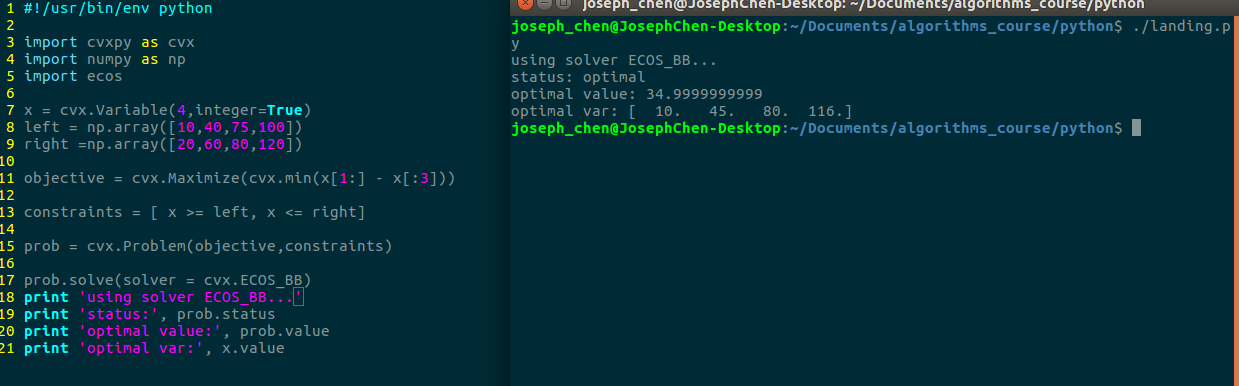
\includegraphics[width=.8\textwidth]{work4/landing}
 \end{figure}
